%% Generated from VALIDATION.md by scripts/md_to_latex.py - edit the Markdown, then re-run the script.
%% Compile with XeLaTeX or LuaLaTeX (e.g. tectonic VALIDATION.tex).
\documentclass[10pt,a4paper]{article}
\usepackage[margin=2cm]{geometry}
\usepackage{fontspec}
\setmainfont{DejaVuSerif.ttf}[BoldFont=DejaVuSerif-Bold.ttf, ItalicFont=DejaVuSerif-Italic.ttf,
  BoldItalicFont=DejaVuSerif-BoldItalic.ttf, Scale=0.92]
\setmonofont{DejaVuSansMono.ttf}[BoldFont=DejaVuSansMono-Bold.ttf, Scale=0.85]
\usepackage{graphicx,longtable,array,enumitem,fvextra,xcolor}
\usepackage[hidelinks]{hyperref}
\usepackage{xurl}
\setlist{nosep,leftmargin=1.4em}
\setlength{\parindent}{0pt}
\setlength{\parskip}{0.5em}
\renewcommand{\arraystretch}{1.2}
\begin{document}

{\LARGE\bfseries Cabin\_Noise: the validation cases and why they were chosen\par}\bigskip

\textbf{Date:} 2026-11-03. \textbf{Cases:} \texttt{cabin\_\allowbreak{}noise/\allowbreak{}data/\allowbreak{}validation/\allowbreak{}cases.\allowbreak{}yaml}. \textbf{Figures:} \texttt{docs/\allowbreak{}figures/\allowbreak{}}, regenerated by \texttt{scripts/\allowbreak{}make\_\allowbreak{}doc\_\allowbreak{}figures.\allowbreak{}py}. They are the same plots the GUI's Validation tab draws.

This document explains:

\begin{itemize}
\item what each case checks;
\item which block of the pipeline it tests;
\item why that data set was chosen;
\item what the result says.
\end{itemize}

METHOD.md gives the equations, VERIFICATION.md the unit-test checks, and \texttt{cases.\allowbreak{}yaml} the exact criteria, dates and recorded results.

\section*{1. The pipeline}

Every block follows one published low-fidelity paper:

\begin{center}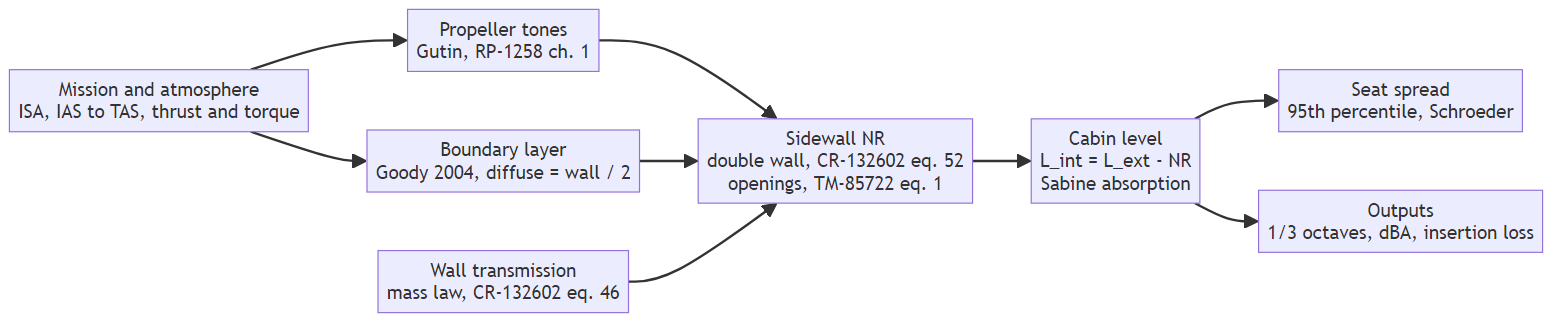
\includegraphics[width=\linewidth,height=0.3\textheight,keepaspectratio]{../figures/mermaid/VALIDATION-c2f776576b.png}\end{center}

The noise reduction (NR) block carries most of the physics. Its inputs are:

\begin{center}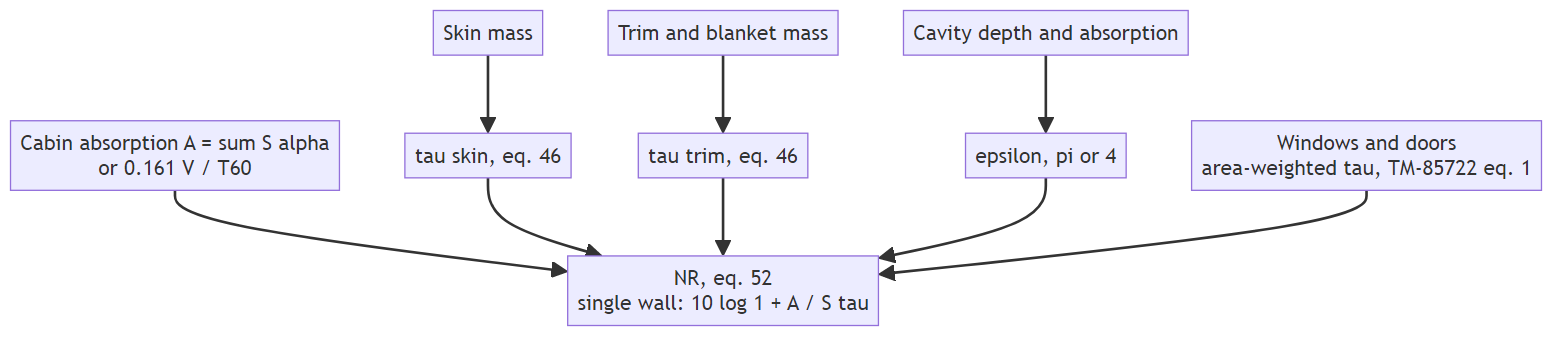
\includegraphics[width=\linewidth,height=0.3\textheight,keepaspectratio]{../figures/mermaid/VALIDATION-4c4549baac.png}\end{center}

\section*{2. Two kinds of case}

\begin{center}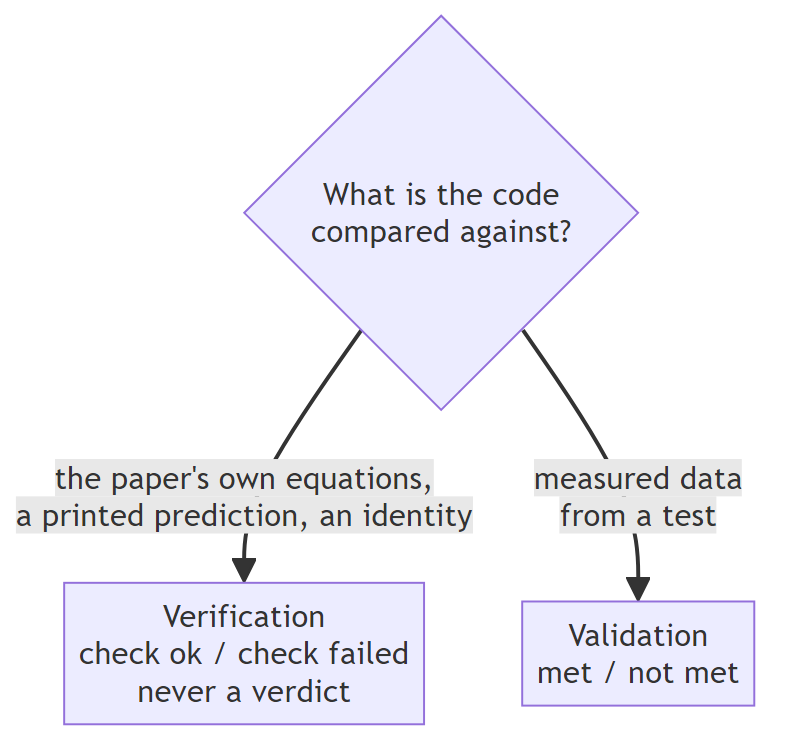
\includegraphics[width=\linewidth,height=0.3\textheight,keepaspectratio]{../figures/mermaid/VALIDATION-2e6da6e352.png}\end{center}

\textbf{Verification} asks whether the code does exactly what the paper says. It is checked against:

\begin{itemize}
\item the paper's equation solved another way;
\item a printed worked example.
\end{itemize}

\textbf{Validation} asks how close the paper's method comes to a measurement. A miss is an acceptable result for a low-fidelity tool. It is recorded with its cause, and never tuned away.

Every case follows the same order:

\begin{center}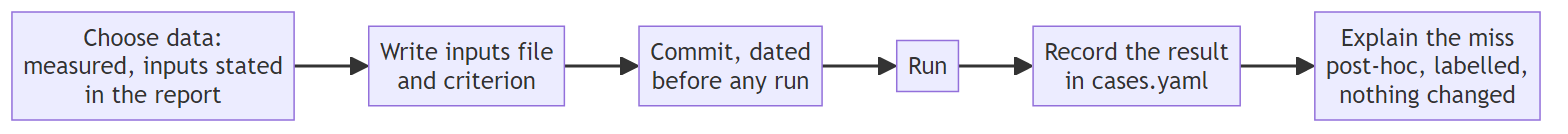
\includegraphics[width=\linewidth,height=0.3\textheight,keepaspectratio]{../figures/mermaid/VALIDATION-bf8e5c1bec.png}\end{center}

\textbf{The criterion for validation cases:} at least 75 \% of the points in range must lie within ±6 dB. This is the low-fi policy of 2026-11-02, written for design trades rather than point accuracy. V4a keeps its original max-error criterion of 3 dB.

\textbf{Why a data set qualifies:}

\begin{enumerate}
\item \textbf{Measured, not predicted.} A printed prediction can only be a verification target, as V2p is.
\item \textbf{Inputs stated.} Every input the method needs is printed in the report, or is a documented assumption committed before the run.
\item \textbf{It isolates a block.} The best case tests one block with the others removed: a lab panel tests the wall alone, and a measured exterior removes the source. End-to-end cases come last.
\item \textbf{Independent.} It is not the data a model change was motivated by. For example, the repeat flights of CR-178004 are not an independent check of flight 3.
\end{enumerate}

\section*{3. Which case tests which block}

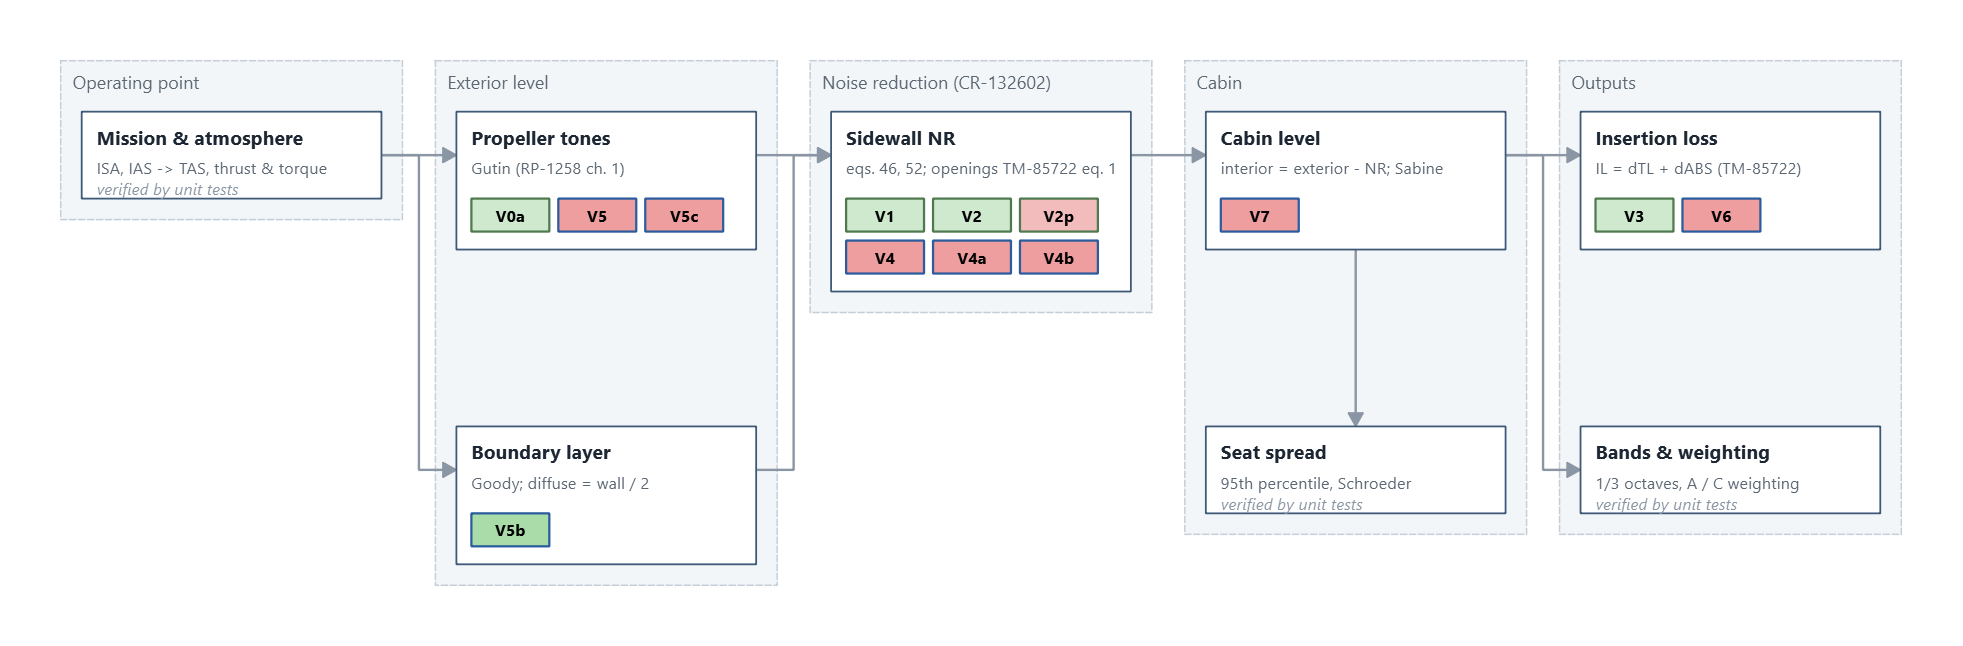
\includegraphics[width=0.8\linewidth]{../figures/map.png}

\begin{center}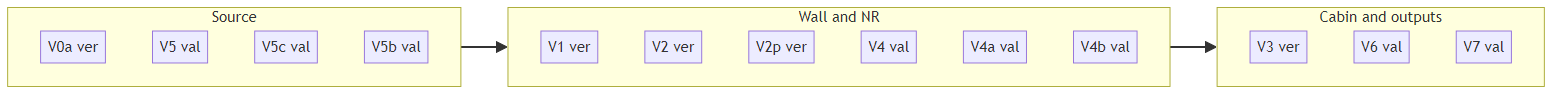
\includegraphics[width=\linewidth,height=0.3\textheight,keepaspectratio]{../figures/mermaid/VALIDATION-884fc2440a.png}\end{center}

\section*{4. Verification cases}

{\small
\begin{longtable}{>{\raggedright\arraybackslash}p{0.031\linewidth}>{\raggedright\arraybackslash}p{0.274\linewidth}>{\raggedright\arraybackslash}p{0.274\linewidth}>{\raggedright\arraybackslash}p{0.149\linewidth}>{\raggedright\arraybackslash}p{0.121\linewidth}}
\hline
\textbf{Case} & \textbf{Checks} & \textbf{Why} & \textbf{Result} & \textbf{Figure} \\
\hline
\endhead
V0a & Gutin's closed form against direct quadrature of the rotating-dipole integral it is derived from & The closed form (Bessel function) is where an implementation slip would hide & check ok, 2e-12 dB & \href{../figures/V0a.png}{V0a} \\
V1 & CR-132602 eq. 46 against the 0-90 deg integral of eq. 45 & Eq. 46 is the closed form of that integral; every wall in the tool uses it & check ok, 9e-10 dB & \href{../figures/V1.png}{V1} \\
V2 & CR-132602 eq. 52 against a numeric solution of the power balance eq. 47 & Eq. 52 is derived from eq. 47. This check also settles the eq. 53 misprint (2/eps against 4/eps) & check ok, 7e-15 dB & \href{../figures/V2.png}{V2} \\
V3 & The pipeline's insertion loss against TM-85722's IL = dTL + dABS & It checks that openings and absorption are wired the way TM-85722 splits them & check ok, 0.28 dB (the "1 +" term) & \href{../figures/V3.png}{V3} \\
V2p & CR-132602 Fig. 14 reproduced from the report's stated inputs & It is the paper's only printed worked example of the NR method: the whole NR block, end to end & \textbf{check failed}, 3.3 dB & \href{../figures/V2p.png}{V2p} \\
\hline
\end{longtable}}

\textbf{V2p in more detail.} The single wall comes out 2.1-3.3 dB below Fig. 14, but with the right shape.

\begin{itemize}
\item The report computed Fig. 14 with eq. 53, which keeps the area ratio S5/S2. It never states that ratio.
\item A post-hoc S5/S2 = 2 closes the gap to within 0.3 dB. That makes the failure a missing input, not a code error, but the recorded result stays "failed".
\item The double-wall curve needs the blanket mass, which is not printed, so it is drawn as information only.
\end{itemize}

\section*{5. Validation cases (measured data)}

\subsection*{Wall and NR}

\textbf{V4: lab TL of the prop-plane treated panel.} Not met, 5/11 bands. \href{../figures/V4.png}{Figure}

\begin{itemize}
\item \textbf{Data:} NASA TM-85722 Fig. 18 and Table I, a Commander 695A sidewall panel measured in the lab.
\item \textbf{Why chosen:} the lab test removes the source and the cabin, so the wall formula is tested alone. The prop-plane layup is the only one whose mass Table I fixes unambiguously.
\item \textbf{Result:} within 3 dB up to 250 Hz. From 315 Hz up it is 6-13 dB low: the septa and barrier on fiberglass act as a second wall, which a single limp wall cannot show.
\end{itemize}

\textbf{V4a: bare cylinder, reverberant NR.} Not met, max 16.5 dB. \href{../figures/V4a.png}{Figure}

\begin{itemize}
\item \textbf{Data:} NASA TP-1964 Fig. 8.
\item \textbf{Why chosen:} it is the simplest structure with measured NR. It has a single wall, no trim, and a measured T60, so it tests the single-wall form with the room term.
\item \textbf{Result:} below about 1 kHz the mass law gives 10-45 dB less NR than measured: the curved shell is stiffness-controlled below its ring frequency (3.3 kHz), which a flat limp wall cannot show. Above 2 kHz the code's NR keeps rising while the measured NR dips toward the ring frequency.
\end{itemize}

\textbf{V4b: stiffened, trimmed cylinder, reverberant NR.} Not met, 5/19 bands. \href{../figures/V4b.png}{Figure}

\begin{itemize}
\item \textbf{Data:} NASA CR-3813 Fig. E-22.
\item \textbf{Why chosen:} it tests the double wall (eq. 52) with trim, and every input is printed in CR-3813.
\item \textbf{Result:} 9-17 dB low at 63-160 Hz (the same stiffness-controlled shell as V4a), within ±6 dB at 200-630 Hz, and 14-22 dB high above 800 Hz, where the double wall rises faster than the measurement. CR-3813 reports that PAIN also overpredicted this case at high frequency.
\end{itemize}

\subsection*{Source}

\textbf{V5: flight exterior tones at the fuselage.} Not met, 65/101. \href{../figures/V5.png}{Figure}

\begin{itemize}
\item \textbf{Data:} NASA CR-178004 App. A, flight 3.
\item \textbf{Why chosen:} it is the measured source level on the same aircraft as V6 and V7, so the source can be judged before the cabin.
\item \textbf{Result:} mean -3.3 dB. BPF1 is close, and BPF2 and BPF3 fall 6-13 dB low. Gutin is a far-field formula, and the microphone is near the tip.
\end{itemize}

\textbf{V5c: static near-field tones.} Not met, 15/52. \href{../figures/V5c.png}{Figure}

\begin{itemize}
\item \textbf{Data:} NACA Report 996 Figs. 12 and 14.
\item \textbf{Why chosen:} it is a different propeller, static and in the lab, so it checks Gutin independently of the flight data.
\item \textbf{Result:} errors up to 47 dB. The points are at d/D = 0.083, deep in the near field where Gutin's far-field form fails.
\end{itemize}

\textbf{V5b: boundary-layer pressure, 800 Hz - 5 kHz.} \textbf{Met}, 265/323. \href{../figures/V5b.png}{Figure}

\begin{itemize}
\item \textbf{Data:} NASA CR-178004 App. D, flight 3.
\item \textbf{Why chosen:} above 800 Hz the report attributes the exterior level to the boundary layer, which isolates Goody's spectrum.
\item \textbf{Result:} mean +2.7 dB.
\end{itemize}

\subsection*{Cabin and outputs}

\textbf{V6: fiberglass insertion loss in flight.} Not met, 372/519 (72 \%). \href{../figures/V6.png}{Figure}

\begin{itemize}
\item \textbf{Data:} NASA CR-178004 App. J, flights 3 and 4.
\item \textbf{Why chosen:} relative trades are the tool's intended use. The insertion loss cancels most of the absolute source error.
\item \textbf{Result:} close to the criterion (75 \% needed). The largest misses (up to +22 dB) are bands where the measured IL is near zero or negative, which a passive treatment model cannot give; the report cites structure-borne components there.
\end{itemize}

\textbf{V7: cabin tones, driven by the measured exterior.} Not met, 1/108. \href{../figures/V7.png}{Figure}

\begin{itemize}
\item \textbf{Data:} NASA CR-178004 App. B, flight 3.
\item \textbf{Why chosen:} the exterior is measured, not predicted, so the case tests NR and cabin in flight without the source error.
\item \textbf{Result:} mean +17.9 dB. The blade passage frequency (78 Hz) lies far below half the fuselage's ring frequency, where CR-132602 itself says its mass-law wall is not valid.
\end{itemize}

\textbf{Summary:} 1 of 8 validation cases met. Every miss lies where its paper's own stated limit puts it:

\begin{itemize}
\item below about half the ring frequency for the mass-law wall (V4a, V4b, V7);
\item the double-wall rise, missing from a single limp wall (V4) and too strong in eq. 52 at high frequency (V4b);
\item the near field for Gutin (V5, V5c).
\end{itemize}

The tool's use is therefore relative trades at mid and high frequency, not absolute tone levels at the blade passage frequency.

\section*{6. Data considered and not used}

{\small
\begin{longtable}{>{\raggedright\arraybackslash}p{0.392\linewidth}>{\raggedright\arraybackslash}p{0.548\linewidth}}
\hline
\textbf{Data} & \textbf{Why not used} \\
\hline
\endhead
TM-85722 Fig. 18, bare-panel curve & It is a calculation, not a measurement. \\
TM-85722 Fig. 18, roof and aft-sidewall layups & Fig. 17 cannot be read for which septa they carry, so their mass is not fixed. They are digitized in \texttt{V4.\allowbreak{}csv} but not compared. \\
CR-132602 Fig. 14 & It is a prediction. It is used as verification (V2p), not validation. \\
CR-178004 flights 1, 2 and 4 (App. A) & Repeat flights of flight 3's conditions, so not an independent check. Flight 4 is used only as V6's treated case. \\
CR-3813 Fig. E-16 (T1/T2 interior levels) & It needs the measured exterior field as a source override, and the trim inputs are incomplete. \\
TP-2444 Figs. 17, 19 & The analysis bandwidth is not stated, and the trim inputs are incomplete. \\
CR-172428 App. B & It holds a program's predictions (PAIN's), not measurements. \\
CR-172490 Fig. 15 & Sharp's double-panel prediction: another method, so verification at most. \\
\hline
\end{longtable}}

\textbf{Retired cases.} V0b, V0c, V4c, V4d and V5d tested models removed in the 2026-11-02 restructure (scattering, box-mode seats, stiffened bays, limp blankets, blade-geometry source). Their records are in git up to commit 1c2c8fe; see METHOD.md sec. 3.

\section*{7. Regenerating the figures}

\begin{Verbatim}[breaklines,fontsize=\small,frame=single,rulecolor=\color{gray}]
.venv/Scripts/python scripts/make_doc_figures.py
\end{Verbatim}

The script runs every case, which takes a few minutes, and saves one PNG per case that has a curve (every case) plus the map to \texttt{docs/\allowbreak{}figures/\allowbreak{}}. Each case figure has three panels:

\begin{itemize}
\item code (line) against reference (markers), with the acceptance band shaded;
\item the error, with ±target;
\item predicted against reference, on a 1:1 line.
\end{itemize}

Each panel has a legend naming its curves (code, the reference and its source, the acceptance band, the target lines, the 1:1 line, and any information curves). The caption below them gives the statistics over the points the verdict counts.

\end{document}
